\chapter{Introduction}

\section{Programming and working with Data in the Time of AI}

\subsection{Integrating AI into Forecasting and Modeling: A Strategic Transformation}

Artificial Intelligence (AI) is not just an enhancement to traditional forecasting and modeling—it is increasingly becoming a \emph{core component} of next-generation weather and climate prediction systems. Some traditional methods will be replaced by AI-driven approaches, while others will be hybridized with AI for better efficiency and accuracy. AI enables \emph{learning directly from observations}, either by improving data assimilation techniques or solving the data to forecasting task by end-to-end learning.

This section presents a structured transformation strategy for adopting AI-based forecasting, model development, and service automation.

\subsubsection{Building AI Expertise with Python and AI Workflows}
To effectively integrate AI, we must ensure our teams are skilled in both AI methods and operational workflows. Our approach includes:
\begin{itemize}[itemsep=1pt,topsep=3pt]

    \item Establishing structured learning paths for key AI techniques relevant to \emph{weather and climate modeling}.
    \item Using Python libraries such as \emph{numpy}, \emph{eccodes}, \emph{netcdf}, and \emph{xarray} for handling large meteorological datasets.
    \item Training teams in machine learning frameworks such as \emph{TensorFlow}, \emph{PyTorch}, and \emph{Hugging Face Transformers}.
    \item Setting up \emph{end-to-end AI workflows} in Jupyter-based environments, covering data ingestion, training, validation, and inference.
    \item Encouraging collaboration between \emph{meteorologists, model developers, and AI experts} to foster cross-disciplinary innovation.
\end{itemize}

\subsubsection{Replacing and Hybridizing Forecasting Systems with AI}
Some forecasting components will be fully \emph{replaced by AI}, while others will integrate AI as a \emph{hybrid solution}. Key shifts include:
\begin{itemize}[itemsep=1pt,topsep=3pt]
    \item \emph{AI-Based Nowcasting}: AI-driven short-term weather predictions using real-time observational data (e.g., satellite, radar, sensors), enhancing or replacing conventional nowcasting techniques.
    \item \emph{Neural Weather Models}: Deep learning models trained on historical data can generate competitive forecasts at lower computational cost.
    \item \emph{Hybrid AI-NWP Models}: AI enhances physics-based forecasting through bias correction, uncertainty quantification, and ensemble optimization.
    \item \emph{Machine Learning for Subgrid Processes}: AI improves or replaces empirical parameterizations in turbulence, cloud physics, and convection models.
    \item \emph{Automated Impact Forecasting}: AI-driven models provide direct risk assessments for extreme weather events, minimizing reliance on manual interpretation.
\end{itemize}

\subsubsection{AI Forecasting and AI Data Assimilation: New Core Components in the Model Chain}

Traditional numerical weather prediction (NWP) relies on physics-based models, but AI is rapidly becoming an integral part of the \emph{full model chain}, improving both forecasting efficiency and data assimilation.

\paragraph{AI-Based Forecasting}
AI-driven forecasting models are evolving as viable alternatives and enhancements to traditional numerical methods:
\begin{itemize}[itemsep=1pt,topsep=3pt]
    \item \emph{AI-Based Nowcasting}: Rapid, high-resolution short-term forecasting from observational data, improving local prediction accuracy.
    \item \emph{Neural Weather Models}: Machine learning models that approximate NWP output with lower computational requirements.
    \item \emph{Hybrid AI-NWP Models}: AI refining traditional numerical forecasts, enhancing post-processing and uncertainty quantification.
\end{itemize}

\paragraph{AI in Data Assimilation and Learning Directly from Observations}
AI is transforming data assimilation, which is essential for initializing forecasts:
\begin{itemize}[itemsep=1pt,topsep=3pt]
    \item \emph{Machine Learning for Observation Processing}: AI-driven quality control of observational data, filling data gaps and detecting sensor anomalies.
    \item \emph{AI-Based Data Assimilation}: AI improving assimilation processes by optimizing observation ingestion.
		\item \emph{Deep Learning for Data Assimilation}: AI learning complex relationships between observations and model states, accelerating assimilation workflows.
    \item \emph{End-to-End AI Data Ingestion}: Future AI models trained directly on observational datasets, potentially reducing reliance on classical assimilation techniques.
    \item \emph{Self-Learning Systems}: AI dynamically adjusting to new data, improving continuously without manual recalibration.
\end{itemize}

\subsubsection{Using AI for Code Refactoring and Model Development}
AI also modernizes modeling workflows, improving efficiency in research and development:
\begin{itemize}[itemsep=1pt,topsep=3pt]
    \item \emph{Refactoring Legacy Code}: AI-assisted tools improving \emph{Fortran, C++, and Python} models for better maintainability and performance.
    \item \emph{Automated Model Optimization}: AI tuning hyperparameters and optimizing computational performance.
    \item \emph{AI-Assisted Scientific Discovery}: AI identifying new climate and weather patterns in large datasets.
    \item \emph{AI-Generated Documentation and Testing}: Automating documentation and generating validation tests for numerical models.
\end{itemize}

\subsubsection{Transforming Services and User Interaction with AI}
AI enables new ways to deliver weather and climate services, improving \emph{automation, personalization, and accessibility}:
\begin{itemize}[itemsep=1pt,topsep=3pt]
    \item \emph{AI-Generated Weather Reports}: Natural language generation models translating raw data into meaningful insights for different user groups.
    \item \emph{Conversational Forecasting Assistants}: AI chatbots and voice assistants allowing users to interactively query weather and climate predictions.
    \item \emph{Real-Time Impact Forecasting}: AI models directly linking weather forecasts to risks in agriculture, energy, transportation, and disaster management.
    \item \emph{AI-Powered Data Visualization}: Interactive AI tools allowing users to explore, manipulate, and interpret complex weather datasets.
\end{itemize}

\subsubsection{A Clear Migration Strategy for AI Transformation}
To successfully integrate AI while maintaining operational stability, we adopt a \emph{structured migration strategy}:
\begin{enumerate}[itemsep=1pt,topsep=3pt]
    \item \emph{AI Readiness Assessment}: Identify areas where AI provides the highest impact while ensuring compatibility with existing workflows.
    \item \emph{Pilot AI Replacements}: Test AI-based forecasting models in parallel with traditional methods before full adoption.
    \item \emph{Hybrid Deployment Strategy}: Introduce AI-driven improvements in \emph{stages}, ensuring fallback options are in place.
    \item \emph{AI Validation and Trust Building}: Develop transparent evaluation metrics for AI models to ensure trust and reliability.
    \item \emph{Workforce Training and Knowledge Transfer}: Enable teams to transition smoothly from traditional methods to AI-driven solutions.
    \item \emph{Continuous AI Governance}: Establish guidelines for AI model retraining, performance monitoring, and ethical considerations.
\end{enumerate}


\subsubsection{Limitations and Responsible Use of AI}

While AI offers transformative opportunities in forecasting, modeling, and service delivery, it is crucial to acknowledge its current limitations and apply it with scientific caution:
\begin{itemize}[itemsep=1pt,topsep=3pt]
    \item \emph{Data Requirements}: Most AI models rely on large, high-quality datasets and perform poorly in data-sparse or non-stationary environments.
    \item \emph{Lack of Physical Consistency}: AI predictions may violate conservation laws or produce unrealistic results in rapidly evolving scenarios.
    \item \emph{Limited Interpretability}: Unlike traditional models, many AI systems operate as black boxes, making it difficult to understand or trace their internal reasoning.
    \item \emph{Bias and Overfitting}: Biased or unbalanced training data can lead to flawed predictions, while overfitting to historical data may reduce adaptability to changing climate conditions.
    \item \emph{Need for Rigorous Validation}: AI models must be continuously monitored, validated, and benchmarked to ensure stability, fairness, and scientific reliability. Validation needs metrics and scores beyond traditional forecasting metrics. 
    \item \emph{Complementary Role}: AI should be seen as an enhancement to—not a replacement for—physics-based modeling, supporting a hybrid approach for trustworthy innovation.
\end{itemize}

By following this transformation roadmap, we ensure that AI adoption is \emph{structured, scalable, and scientifically sound}, positioning our forecasting and modeling systems for the future.

%==============================================================================
%
%==============================================================================
\section{General Coding Rules and Strategy}

Our coding principles focus on \emph{maintainability, testability, and automation}. Code should be structured, tested, and versioned properly, ensuring long-term reliability and ease of collaboration.

\subsection{Code Management with Git}
All code is managed in Git, following a structured workflow:
\begin{itemize}[itemsep=1pt,topsep=3pt]
    \item \emph{Repository Structure}: Organize code into well-defined modules, using a clear folder structure (\texttt{src/}, \texttt{tests/}, \texttt{docs/}).
    \item \emph{Branching Strategy}: Use a master/dev/feature branching model:
    \begin{itemize}[itemsep=1pt,topsep=3pt]
        \item \texttt{master}: Production-ready, thoroughly tested.
        \item \texttt{dev}: Integration branch for new features.
        \item \texttt{feature/*}: Short-lived branches for individual tasks, merged via pull requests.
    \end{itemize}
    \item \emph{Commits and Documentation}:
    \begin{itemize}[itemsep=1pt,topsep=3pt]
        \item Each commit should contain \emph{atomic changes} with clear commit messages (\texttt{git commit -m "Refactored data pipeline for efficiency"}).
        \item You might use Git hooks for enforcing style checks (e.g., \texttt{pre-commit} for \texttt{black} and \texttt{flake8}). 
    \end{itemize}
\end{itemize}

\subsubsection{Essential Git Commands and Best Practices}
\emph{Git} is a distributed version control system, enabling efficient collaboration. The following commands cover the most common workflows. We usually employ git via \texttt{gitlab} or \texttt{github}, but you can use it yourself on any linux system, letting your own repo work as a server for you, and do git add/commit/push as with some gitlab installation!

\paragraph{Initializing and Cloning Repositories}
\begin{verbatim}
git init  # Initialize a new Git repository
git clone <repo-url>  # Clone an existing repository
\end{verbatim}

\paragraph{Working with Branches}
\begin{verbatim}
git branch feature-xyz            # Create a new branch
git checkout feature-xyz          # Switch to a branch
git switch -c feature-xyz         # Create and switch to a branch (newer Git versions)
git checkout -b mylocalname origin/reponame  # Track a remote branch with a local name
git merge feature-xyz             # Merge changes into the current branch
git rebase main                   # Reapply commits on top of the main branch
\end{verbatim}


\paragraph{Committing and Pushing Changes}
\begin{verbatim}
git status  # Show modified files
git add .  # Stage all changes
git commit -m "Describe your change"  # Commit changes
git push origin feature-xyz  # Push changes to the remote repository
\end{verbatim}

\paragraph{Syncing and Undoing Changes}
\begin{verbatim}
git pull origin main  # Update the local branch with remote changes
git reset --hard HEAD~1  # Undo the last commit
git checkout -- <file>  # Revert changes to a file before commit
\end{verbatim}

\paragraph{Tracking and Reviewing History}
\begin{verbatim}
git log --oneline --graph --decorate  # View commit history
git diff  # Show uncommitted changes
git blame <file>  # Show line-by-line history of changes
\end{verbatim}

\paragraph{Best Practices for Git Usage}
\begin{itemize}[itemsep=1pt,topsep=3pt]
    \item \emph{Commit frequently}: Avoid large, monolithic commits.
    \item \emph{Write meaningful commit messages}: Summarize what and why, not just how.
    \item \emph{Rebase instead of merge (when appropriate)}: Keeps history linear.
    \item \emph{Use .gitignore}: Prevent unnecessary files from being tracked.
    \item \emph{Pull before pushing}: Avoid conflicts by updating from the remote branch.
    \item \emph{Tag important versions}: Use \texttt{git tag v1.0} for release milestones.
\end{itemize}

\subsubsection{Adding a \texttt{.gitignore} File for LaTeX Projects}

Before committing files to a Git repository, it's important to add a \texttt{.gitignore} file to prevent cluttering the version history for example with automatically generated LaTeX files. These include temporary files, auxiliary logs, and build artifacts that should not be tracked. Here's a recommended \texttt{.gitignore} for LaTeX projects:
\begin{verbatim}
# LaTeX intermediate and output files
*.aux
*.bbl
*.blg
*.brf
*.fdb_latexmk
*.fls
*.idx
*.ilg
*.ind
*.lof
*.log
*.lot
*.nav
*.out
*.pdf
*.snm
*.synctex.gz
*.toc
*.vrb
*.xdv

# Editor backup files
*~
*.swp
.DS_Store
\end{verbatim}
This ensures that only the actual source files (e.g., \texttt{.tex}, \texttt{.bib}, \texttt{.sty}, images, and configuration files) are tracked in your repository.

\subsubsection{Best Practices for Repository Management}

\begin{itemize}
  \item \emph{Do not commit large binaries or large images into a GitLab or any other code repository!}  
  \item \emph{Keep project-related materials (e.g., PowerPoint presentations) in separate repositories from code development!} 
	
	Usually, it is a good idea to have your project repo with branches in a place where storage limitations are not important. You can use a local git repo to make sure your own versions on different computers are well synchronized, and clone and push into a central space on some linux server. Use gitlab or github to manage code repos. 
  \item \emph{Do not store measurement or model data in a Git repository!}  
  \item Manage data instead in accessible folders with a clear and documented structure, or store it in a database environment.  
\end{itemize}

\subsection{Managing Multiple Git Repositories for AI Development}

AI-based applications for weather, climate, and environmental forecasting often involve multiple interconnected repositories, such as core models, data pipelines, and frontend applications. Efficiently managing and synchronizing these repositories is essential, especially in large-scale initiatives like the \emph{EUMETNET E-AI Programme on Artificial Intelligence and Machine Learning for Weather, Climate, and Environmental Applications} or the \emph{DWD AI Center}. When we want to work both with e.g.\ DWD repos, MeteoFrance repos, AnemoI repos and your local repos, a careful repo management is in order. 

To facilitate multi-repo workflows, we either use lean and elementary scripts such as \texttt{gitall} or we employ a combination of \texttt{meta} (for managing multiple repositories as a single unit) and \texttt{git worktree} (for handling multiple branches efficiently).

%==============================================================================
%
%==============================================================================
\paragraph{Elementary Git Repository Management Script}

To streamline the handling of multiple Git repositories in a single parent folder, we provide the script \texttt{gitall.sh} (located in \texttt{\scriptsize ./scripts}). Its key features and usage recommendations are:

\begin{itemize}
  \item \emph{Location:} The script is located in the \texttt{./scripts} directory.
  \item \emph{Function:} It checks the status of all Git repositories or updates them with \texttt{git pull} commands.
  \item \emph{Usage examples:}
  \begin{itemize}
    \item \texttt{./gitall.sh pull} – Pulls the latest changes in all repositories.
    \item \texttt{./gitall.sh s} – Shows the Git status for all repositories.
    \item \texttt{./gitall.sh pull s} – Pulls and then shows the status.
  \end{itemize}
  \item \emph{Recommendation:} Create a symbolic link (e.g., \texttt{ln -s ./scripts/gitall.sh ~/bin/gitall}) to call it globally.
  \item \emph{Documentation:} Detailed usage information is included as comments at the top of the script.
\end{itemize}
The script is easily extensible to your particular needs. 

\paragraph{Organizing Repositories with Meta} 
The package \texttt{meta} enables structured management of multiple repositories by defining them in a single \texttt{meta.json} file. This allows users to clone, update, and execute commands across all repositories in a unified manner.

\begin{verbatim}
{
  "projects": {
    "eai-tutorials": "https://github.com/eumetnet-e-ai/tutorials.git",
    "eai-toolbox-explore": "https://gitlab.dkrz.de/dwd-ki-zentrum/\
		infrastructure/e-ai_toolbox_explore"
  }
}
\end{verbatim}

With this setup, all repositories can be cloned simultaneously using:
\begin{verbatim}
meta git clone
\end{verbatim}

%==============================================================================
%
%==============================================================================
\subsubsection{Efficient Branch Management with Git Worktree}
For AI research and development, multiple experiments and feature branches often need to be managed simultaneously. Instead of constantly switching branches, \texttt{git worktree} allows separate working directories for each branch.

To create worktrees for feature branches:
\begin{verbatim}
meta exec "git worktree add ../feature-dwd-ai feature-branch"
meta exec "git worktree add ../feature-eai-pipeline feature-branch"
\end{verbatim}

This approach provides a clean way to work on different tasks in parallel without redundant repository clones.

\paragraph{Automation and Best Practices}
To ensure consistency in AI workflows:
\begin{itemize}[itemsep=1pt,topsep=3pt]
    \item Pull updates across repositories with:
    \begin{verbatim}meta exec "git pull origin main"\end{verbatim}
    \item Regularly clean up unused worktrees:
    \begin{verbatim}meta exec "git worktree prune"\end{verbatim}
    \item Store \texttt{meta.json} in version control to ensure reproducibility across teams.
    \item Automate workflows via CI/CD pipelines to test and deploy AI models across repositories.
\end{itemize}

By integrating \lstinline|meta| and \lstinline|git worktree|, the DWD AI Center and EUMETNET E-AI Programme can maintain a structured and efficient workflow, allowing researchers and engineers to focus on AI model development rather than repository management.


%==============================================================================
%
%==============================================================================
\subsection{Testing and Continuous Integration}

To maintain quality, every function and module should have explicit \emph{unit tests}, written with \texttt{pytest}. We encourage a \emph{test-driven development (TDD)} approach where applicable.

\begin{itemize}[itemsep=1pt,topsep=3pt]
    \item \emph{Unit Testing}: Every function should be covered by a test to catch potential bugs early.
    \item \emph{Integration Testing}: Ensure different components interact correctly, particularly in model training and evaluation pipelines.
    \item \emph{Automated Testing}:
    \begin{itemize}[itemsep=1pt,topsep=3pt]
        \item Git push should be able to trigger a \emph{CI/CD pipeline} that runs all tests.
        \item Developers should be able to run \texttt{pytest} locally before committing changes.
        \item Centralized CI testing (e.g., GitHub Actions, GitLab CI/CD, Jenkins) should validate code before deployment.
    \end{itemize}
\end{itemize}

\subsection{Code Quality and Documentation}
Maintaining high code readability and quality is essential. The following standards apply:

\begin{itemize}[itemsep=1pt,topsep=3pt]
    \item \emph{Code Formatting}: Enforce coding standards using \texttt{black} (formatting), \texttt{flake8} (linting), and \texttt{mypy} (type checking).
    \item \emph{Pre-Commit Hooks}: Automate checks to prevent incorrect code from being committed.
    \item \emph{Documentation}:
    \begin{itemize}[itemsep=1pt,topsep=3pt]
        \item Every function and class should include \emph{docstrings} in \texttt{Google} or \texttt{NumPy} format.
        \item API documentation should be maintained using \texttt{mkdocs} or \texttt{Sphinx}.
    \end{itemize}
\end{itemize}

\subsection{Reproducibility and Environment Management}
To ensure consistent execution across different systems:

\begin{itemize}[itemsep=1pt,topsep=3pt]
    \item \emph{Dependency Management}:
    \begin{itemize}[itemsep=1pt,topsep=3pt]
        \item Use virtual environments such as \texttt{venv}, \texttt{Poetry}, or \texttt{Pipenv} for managing dependencies.
        \item Store dependencies explicitly in \texttt{pyproject.toml} (Poetry) or \texttt{requirements.txt} (pip).
    \end{itemize}
    \item \emph{Containerization}:
    \begin{itemize}
        \item Use Docker to provide isolated, reproducible environments.
        \item Maintain \emph{pre-configured environments} for development and production.
    \end{itemize}
\end{itemize}

\subsection{Automated Workflows and Continuous Deployment}
Automation is key to ensuring reliability and scalability:

\begin{itemize}[itemsep=1pt,topsep=3pt]
    \item \emph{CI/CD Pipelines}: Tests, builds, and deployments should at least in principle be fully automated, meaning that necessary human based evaluation and reviews are built into an automated process which is thoroughly tested. 
    \item \emph{Model Retraining and Monitoring}: Machine learning models will probably be retrained on a regular basis, with performance monitoring to track drift.
    \item \emph{Version Control for Models}: Every trained model should be versioned for reproducibility.
\end{itemize}

We remark that most of these steps are standard in the framework of \emph{Numerical Weather Prediction}, where code management for models and data assimilation code has a long tradition. Also, running a very organized process including
\begin{itemize}[itemsep=1pt,topsep=3pt]
\item \textbf{code development},  
\item small and large-scale \textbf{testing}, 
\item \textbf{evaluation} and \textbf{verification}, 
\item \textbf{decision making} based on the results and 
\item deployment through an operational system with \textbf{parallel routine} and 
\item \textbf{routine} runs based on ecflow schedulers 
\end{itemize}
is best-practice in NWP centres. At DWD, we run a weekly \emph{routine meeting} where evaluation results and decisions are made for the NWP forecasting system. Scripting systems for full-scale NWP experiments are available both for fast development and routine-type testing and deployment. AI applications can seamlessly be integrated into this approach, which guarantees quality ensurance and flexiblity at the same time. 

\subsection{Basic Coding Principles}
\begin{itemize}[itemsep=1pt,topsep=3pt]
    \item Use meaningful variable names and keep functions concise.
    \item Follow PEP8 for consistent Python code style.
    \item Avoid hardcoded values; instead, use configuration files.
    \item Ensure all functions include a well-defined docstring.
\end{itemize}

\subsection{Git and Collaboration Best Practices}
To maintain a clean and organized codebase:

\begin{itemize}[itemsep=1pt,topsep=3pt]
    \item Follow a structured Git workflow using \texttt{main}, \texttt{dev}, and \texttt{feature/*} branches.
    \item Ensure commits are atomic, with a clear description of changes.
    \item Use Git hooks to enforce style checks automatically before committing.
\end{itemize}

\subsection{Testing and Quality Assurance}
Before merging code:

\begin{itemize}[itemsep=1pt,topsep=3pt]
    \item Every function should have a corresponding unit test.
    \item Tests should be run locally before pushing changes to Git.
    \item CI/CD pipelines must validate all code changes with unit and integration tests.
\end{itemize}

\subsection{Deployment and Reproducibility}
To ensure stable production releases:

\begin{itemize}[itemsep=1pt,topsep=3pt]
    \item No code is merged into \texttt{master} unless all tests pass.
    \item Machine learning models should be retrained periodically with performance monitoring.
    \item Environments should be reproducible using virtual environments with requirements files or Docker containers.
\end{itemize}

%==============================================================================
%
%==============================================================================
\subsubsection{Structure of the DWD AI Centre}

We note that the Structure of the DWD AI Centre as shown in Figure \ref{fig:ai_centre_structure} is higly dynamic, with projects and repos being in a process of setup and consolidation. The following graphics provides a snapshot and example layout as currently pursued. 

\begin{figure}[h]
  \centering
  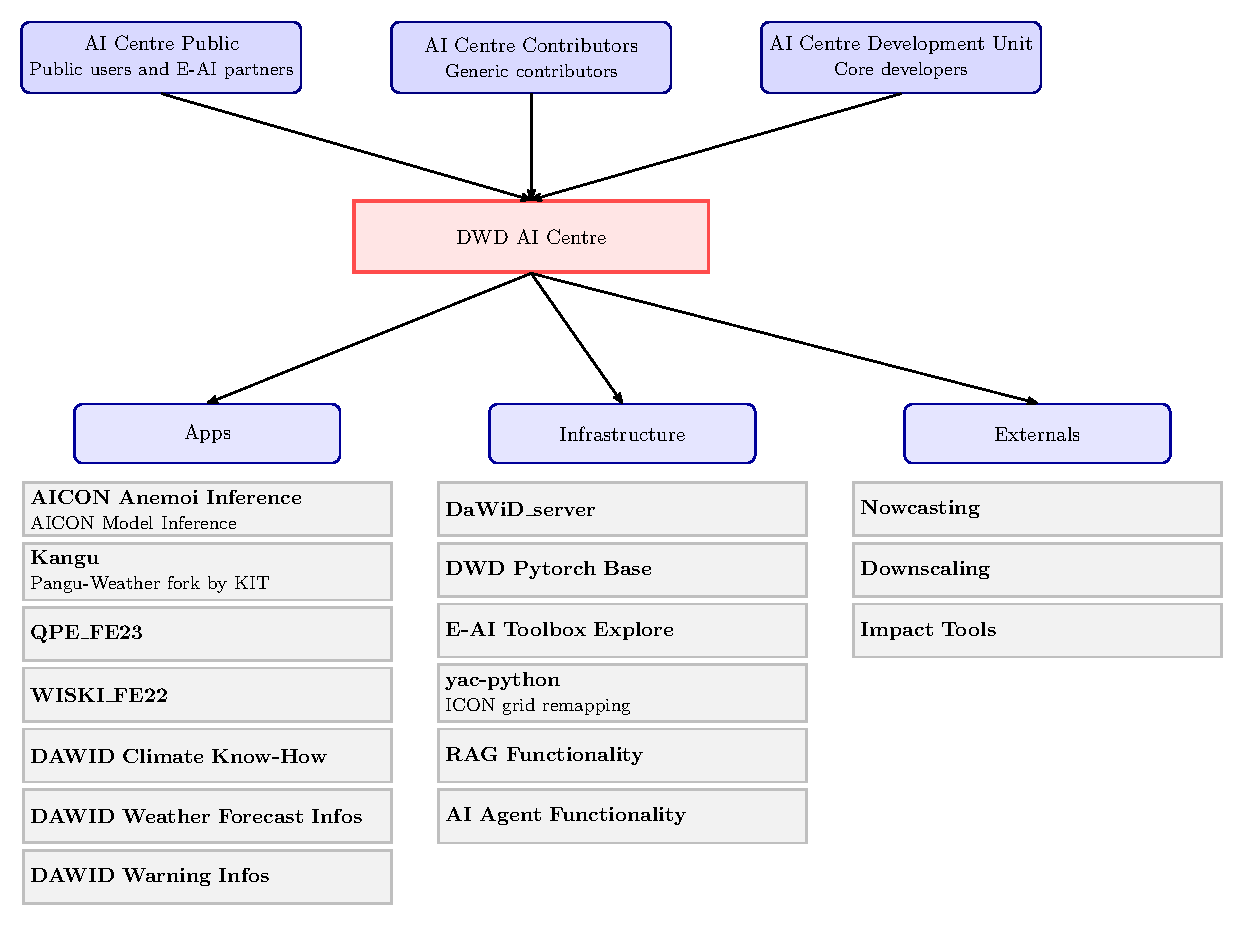
\includegraphics[width=\textwidth]{chapters/ai_centre_graphics.pdf}
  \caption{Organizational and technical structure of the DWD AI Centre repositories.}
  \label{fig:ai_centre_structure}
\end{figure}

\begin{itemize}
  \item The DWD AI Centre connects internal development units, contributors, and public users to shared infrastructure and applications.
  \item The repository structure is grouped into \emph{Apps}, \emph{Infrastructure}, and \emph{Externals}, each containing specific projects for modeling, processing, and integration.
  \item The central node acts as the coordination hub, linking various AI-driven tools with operational workflows and collaborative partners.
\end{itemize}



%==============================================================================
%
%==============================================================================
\section{6 Days Python and AI}

\subsection{Schedule}
\noindent The following table provides an overview of the tutorial structure, covering key topics in Python programming, artificial intelligence, and machine learning for applications in weather, climate, and environmental sciences. The tutorial is designed as a structured six-day course, with each day focusing on a specific theme. The content progresses from fundamental Python concepts and data handling to advanced AI techniques such as large language models (LLMs), retrieval-augmented generation (RAG), and AI-driven forecasting. We introduce many practical applications, and advanced topics including AI data assimilation, model emulation, and AI-enhanced operational workflows. Each day consists of multiple modules, ensuring a comprehensive and hands-on learning experience.

%------------------------------------------------------------------------------
% 
%------------------------------------------------------------------------------
\begin{longtable}{|c|p{5cm}|p{8cm}|}
\hline
\rowcolor{headerblue} \textbf{Chapter} & \textbf{Title} & \textbf{Sections} \\
\hline
\endhead
\hline
\endfoot

%------------------------------------------------------------------------------
\multicolumn{3}{|c|}{\cellcolor{headerblue} \textbf{Day 1: Python as Workhorse}} \\ \hline
\rowcolor{lightblue} 1  & Python Basics & Python syntax, data types, control structures, functions, file I/O \\ \hline
2  & Jupyter Notebooks, APIs and Servers & Setting up Jupyter, working with APIs, creating servers \\ \hline
\rowcolor{lightblue} 3  & Eccodes for Grib, Opendata, NetCDF, Observations, Visualization & GRIB and NetCDF handling with eccodes, accessing OpenData, visualization techniques \\ \hline

%------------------------------------------------------------------------------
\multicolumn{3}{|c|}{\cellcolor{headerblue} \textbf{Day 2: AI/ML Basic Introduction}} \\ \hline
\rowcolor{lightblue} 4  & Machine Learning Basics & Supervised and unsupervised learning, data preprocessing, model evaluation \\ \hline
5  & Neural Network Architectures & Feedforward Networks, Graph Neural Networks, Convolutional Networks, Transformers \\ \hline
\rowcolor{lightblue} 6  & Large Language Models & LLM network structure, Installing and using Ollama, Python API, Local UI with history \\ \hline

%------------------------------------------------------------------------------
\multicolumn{3}{|c|}{\cellcolor{headerblue} \textbf{Day 3: LLM RAG, Python Packages, Multi-Modality}} \\ \hline
\rowcolor{lightblue} 7  & LLM with Retrieval-Augmented Generation (RAG) & Introduction to RAG, Installing dependencies, Loading and processing documents, Generating embeddings, Using FAISS, Retrieving documents, Response generation \\ \hline
8  & Python Packages & Python Standard Library, Xarray basics, Pandas, SciPy, Scikit-learn \\ \hline
\rowcolor{lightblue} 9  & Multimodal LLMs & Modalities, Integration, Fusion, Cross-Attention, Use Cases, AI Interaction, Data Alignment, Benchmarking \\ \hline

%------------------------------------------------------------------------------
\multicolumn{3}{|c|}{\cellcolor{headerblue} \textbf{Day 4: GPUs, AI Agents, Services and Impact}} \\ \hline
\rowcolor{lightblue} 10 & Using GPUs for Training Applications & Checking GPU availability, Installing dependencies, Exploring GPU tensors, Training models on GPU, Comparing CPU vs GPU \\ \hline
11 & Agents and Coding with LLM & Introduction to LLM coding, Agent frameworks, LangChain example, Auto-GPT example \\ \hline
\rowcolor{lightblue} 12 & LLMs for Geosciences, Weather, and Climate & Feature Detection, Weather Reports, Forecast Interpretation, Communication, Impact Forecasting, Decision Support \\ \hline

%------------------------------------------------------------------------------
\multicolumn{3}{|c|}{\cellcolor{headerblue} \textbf{Day 5: LLM Maturity and Operations}} \\ \hline
\rowcolor{lightblue} 13 & MLFlow - Managing and Monitoring Training & Setting up MLFlow, Monitoring Training, Comparing Experiments, Managing Parameters \\ \hline
14 & MLOps - Operations & Principles, Workflow, Deployment, Monitoring, CI/CD, Automation, Reproducibility, Scalability, Kubernetes, Cloud, On-Premise \\ \hline
\rowcolor{lightblue} 15 & Fine-Tuning LLMs & Fine-Tuning, LLMs, Dataset Preparation, Tokenization, LoRA, Reinforcement Learning, Evaluation, Deployment, Scalability \\ \hline

%------------------------------------------------------------------------------
\multicolumn{3}{|c|}{\cellcolor{headerblue} \textbf{Day 6: AI Model and AI Data Assimilation}} \\ \hline
\rowcolor{lightblue} 16 & AnemoI & Overview of AnemoI and its capabilities \\ \hline
17 & Model Emulation and AICON & Emulating weather models with AI, AICON framework \\ \hline
\rowcolor{lightblue} 18 & AI Data Assimilation & AI-driven data assimilation, Applications in numerical weather prediction \\ \hline

%------------------------------------------------------------------------------
% Appendix Section with a Header
%------------------------------------------------------------------------------
\multicolumn{3}{|c|}{\cellcolor{appendixblue} \textbf{Appendix: Background and Additional Topics}} \\ \hline
\rowcolor{lightblue} A1 & Large Language Models - History and Development & History and evolution of LLMs, Key architectures and breakthroughs \\ \hline
A2 & Advanced GPU Utilization & Mixed-precision training, Model parallelism, Efficient GPU scheduling \\ \hline
\rowcolor{lightblue} A3 & Future Trends in AI and Weather Forecasting & Hybrid AI-NWP models, Real-time assimilation, AI-driven extreme event forecasting \\ \hline

\end{longtable}

%==============================================================================
%
%==============================================================================
\subsection{Training Codes}
\noindent To ensure a structured and reproducible learning experience, all training codes are provided \emph{chapter by chapter}. This should allow participants to \emph{easily locate, reference, and execute} the relevant scripts corresponding to specific tutorial sections. 

We have tested the scripts as far as possible for the following computing environments and give specific advice when things were difficult in a particular framework. 

\begin{center}
\begin{figure}[h]
   \centerline{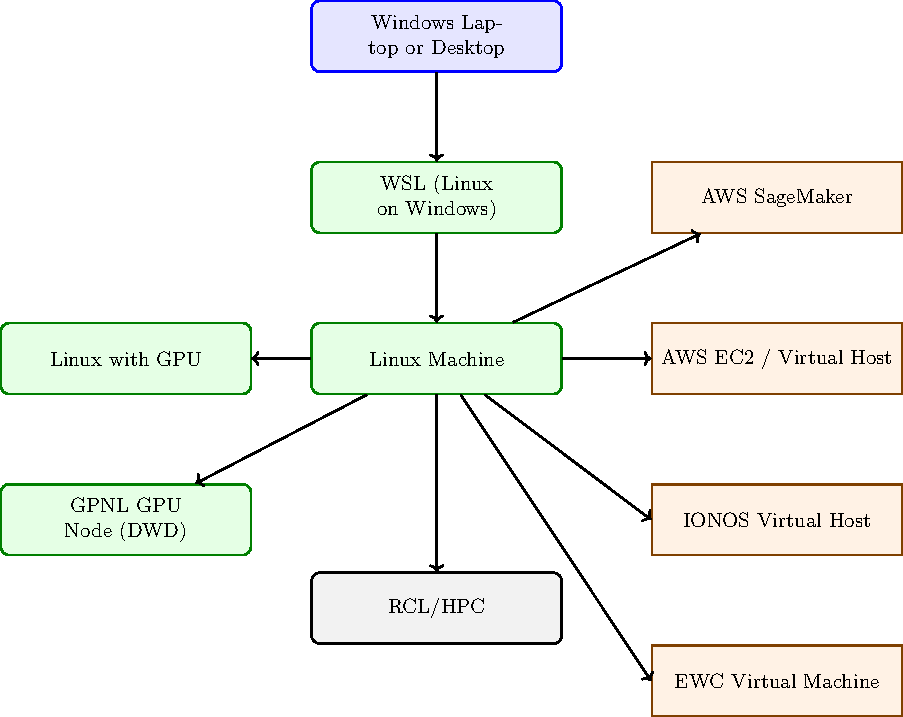
\includegraphics[width=0.8\textwidth]{chapters/computing_environments.pdf}}
	\caption{We want to enable choices and independence of particular solutions or infrastructures.}
\end{figure}
\end{center}%

